\chapter{The ggen Architecture}
\label{ch:architecture}

\section{Foundational Principles}

The ggen architecture rests on three foundational principles that distinguish it from traditional code generators.

\subsection{Ontology as Single Source of Truth}

The core equation of ggen is:

\begin{equation}
A = \mu(O)
\end{equation}

Where $A$ represents generated artifacts (code, configurations, documentation), $O$ represents the RDF ontology specification, and $\mu$ represents the deterministic transformation pipeline.

\begin{theorem}[Determinism Guarantee]
For any well-formed ontology $O$ and transformation configuration $C$, the generated artifacts are uniquely determined:
\[
\forall O, C: \mu(O, C) = \mu(O, C)
\]
\end{theorem}

\subsection{The Five-Stage Pipeline}

ggen implements a five-stage transformation pipeline:

\begin{figure}[h]
\centering
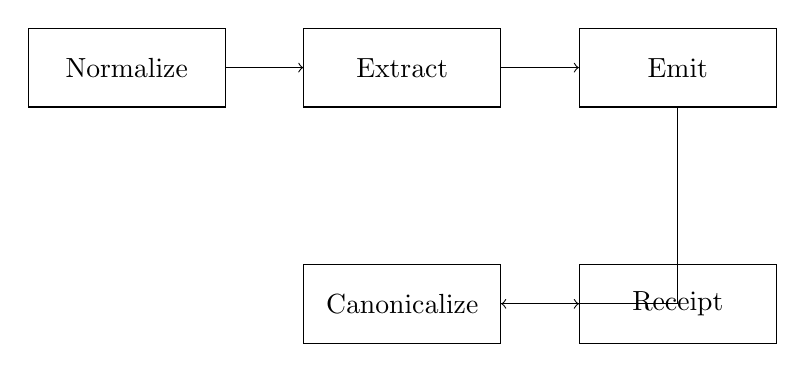
\begin{tikzpicture}[node distance=2cm, auto]
  \node[draw, rectangle, minimum width=2.5cm, minimum height=1cm] (norm) {Normalize};
  \node[draw, rectangle, minimum width=2.5cm, minimum height=1cm, right of=norm, xshift=1.5cm] (extract) {Extract};
  \node[draw, rectangle, minimum width=2.5cm, minimum height=1cm, right of=extract, xshift=1.5cm] (emit) {Emit};
  \node[draw, rectangle, minimum width=2.5cm, minimum height=1cm, below of=extract, yshift=-1cm] (canon) {Canonicalize};
  \node[draw, rectangle, minimum width=2.5cm, minimum height=1cm, right of=canon, xshift=1.5cm] (receipt) {Receipt};

  \draw[->] (norm) -- (extract);
  \draw[->] (extract) -- (emit);
  \draw[->] (emit) |- (canon);
  \draw[->] (canon) -- (receipt);
\end{tikzpicture}
\caption{The ggen five-stage pipeline}
\label{fig:pipeline}
\end{figure}

\begin{enumerate}
\item \textbf{Normalize}: Load and validate RDF, resolve prefixes, expand shortcuts
\item \textbf{Extract}: Execute SPARQL queries to extract generation context
\item \textbf{Emit}: Apply Tera templates to extracted data
\item \textbf{Canonicalize}: Format and standardize generated code
\item \textbf{Receipt}: Generate deterministic proof of transformation
\end{enumerate}

\subsection{Quality Gates and Andon Signals}

ggen integrates Toyota Production System principles through Andon signals:

\begin{table}[h]
\centering
\begin{tabular}{clp{7cm}}
\toprule
\textbf{Signal} & \textbf{Status} & \textbf{Action} \\
\midrule
\textcolor{green}{$\bullet$} & GREEN & All checks pass, proceed safely \\
\textcolor{yellow}{$\bullet$} & YELLOW & Warnings present, investigate before release \\
\textcolor{red}{$\bullet$} & RED & Errors detected, stop immediately \\
\bottomrule
\end{tabular}
\caption{Andon signal definitions}
\label{tab:andon}
\end{table}

\section{The Oxigraph RDF Store}

ggen uses Oxigraph as its RDF substrate, providing:

\begin{itemize}
\item In-memory and persistent storage modes
\item Full SPARQL 1.1 Query and Update support
\item Rust-native performance characteristics
\item Thread-safe concurrent access
\end{itemize}

\subsection{Query Optimization}

SPARQL queries in ggen are optimized through:

\begin{lstlisting}[language=SPARQL,caption={Optimized Entity Query}]
PREFIX ggen: <http://ggen.dev/ontology#>

SELECT ?entity ?name ?type WHERE {
  ?entity a ggen:Entity ;
          ggen:name ?name ;
          ggen:type ?type .
  FILTER(STRSTARTS(STR(?entity), STR(ggen:)))
}
ORDER BY ?name
\end{lstlisting}

\section{Template System Architecture}

\subsection{Tera Template Engine}

ggen employs Tera for template rendering, supporting:

\begin{itemize}
\item Jinja2-compatible syntax
\item Template inheritance and includes
\item Custom filters and functions
\item Compile-time validation
\end{itemize}

\subsection{Template Resolution}

Templates are resolved through a layered system:

\begin{enumerate}
\item Project-local templates (\texttt{.ggen/templates/})
\item Installed pack templates (\texttt{\textasciitilde/.ggen/packs/})
\item Built-in default templates
\end{enumerate}

\section{The Pack System}

Packs encapsulate reusable generation recipes:

\begin{definition}[Pack]
A pack $P = (O_p, T_p, M_p)$ consists of:
\begin{itemize}
\item $O_p$: Base ontology fragments
\item $T_p$: Template collection
\item $M_p$: Metadata and configuration
\end{itemize}
\end{definition}

\subsection{Pack Composition}

Packs compose through union with conflict resolution:

\begin{equation}
P_{composed} = P_1 \cup_{resolve} P_2 \cup_{resolve} \ldots \cup_{resolve} P_n
\end{equation}

\section{Integration Points}

\subsection{CLI Architecture}

The ggen CLI provides the primary interface:

\begin{lstlisting}[language=bash,caption={Core CLI Commands}]
ggen sync              # Regenerate from ontology
ggen validate          # Validate specifications
ggen wizard new        # Create project from NL
ggen pack install      # Install generation pack
\end{lstlisting}

\subsection{Cargo Make Integration}

All ggen operations integrate with Cargo Make for SLO enforcement:

\begin{lstlisting}[language=toml,caption={Cargo Make Integration}]
[tasks.ggen-sync]
command = "ggen"
args = ["sync", "--receipt"]
dependencies = ["validate-ontology"]
\end{lstlisting}

\section{Architectural Invariants}

The following invariants are maintained throughout the system:

\begin{enumerate}
\item \textbf{Ontology Immutability}: Once closed, ontologies are never modified---only regenerated from source
\item \textbf{Template Purity}: Templates are pure functions of their input context
\item \textbf{Receipt Completeness}: Every generation produces a verifiable receipt
\item \textbf{Error Locality}: Errors in specifications cause early failure, never propagate to generated code
\end{enumerate}

\section{Summary}

The ggen architecture provides a solid foundation for specification-driven code generation. The five-stage pipeline ensures deterministic transformation, while quality gates prevent error propagation. This architecture enables wizard commands to generate specifications that flow unchanged through the existing generation infrastructure.
